\documentclass{beamer}

\usepackage{color}
\usepackage{graphicx}
\usepackage{hyperref}
\usepackage{listings}
\usepackage{minted}

\definecolor{dkgreen}{rgb}{0,0.6,0}
\definecolor{gray}{rgb}{0.5,0.5,0.5}
\definecolor{mauve}{rgb}{0.58,0,0.82}

\lstset{frame=tb,
  language=Java,
  aboveskip=3mm,
  belowskip=3mm,
  showstringspaces=false,
  columns=flexible,
  basicstyle={\small\ttfamily},
  numbers=none,
  numberstyle=\tiny\color{gray},
  keywordstyle=\color{blue},
  commentstyle=\color{dkgreen},
  stringstyle=\color{mauve},
  breaklines=true,
  breakatwhitespace=true,
  tabsize=3
}

\title[Intro to Python]{Philosophy and Fundamentals}
\begin{document}
\frame{\titlepage}


\begin{frame}
  \frametitle{Background}
  \begin{enumerate}
    \item Authored by Guido van Rossum
    \item Implemented in 1989, released in 1994
    \item Inspired by programming language \textsc{abc}
    \item Named after comedy series \textit{Monty Python's Flying Circus}
  \end{enumerate}
  \begin{figure}
    \begin{center}
    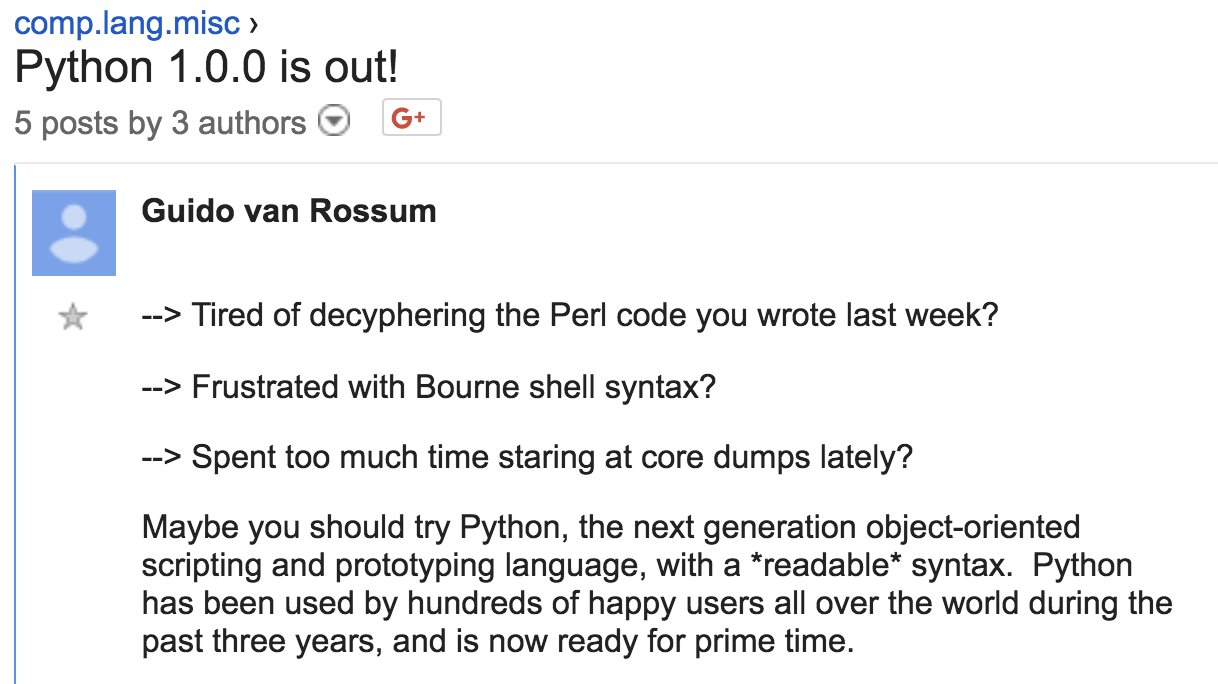
\includegraphics[width=175pt,keepaspectratio]{release.jpg}
    \caption
    {
      Snippet\footnote{\url{www.twitter.com/jakevdp/status/957126964791291905}}
      of Python 1.0.0 Release in 
      1994\footnote
      {
       \url{groups.google.com/forum/?hl=en\#!topic/comp.lang.misc/_QUzdEGFwCo}
      }
    }
    \end{center}
  \end{figure}
\end{frame}


\begin{frame}
  \frametitle{Things You Might Hear\ldots}
  \begin{itemize}
    \item ``Batteries included''
    \item ``We're all adults here''
    \item ``There's only one (obvious) way to do it''
    \item \textsc{tsttcpw} (the simplest thing that could possibly work)
    \item Guido's time machine
    \item Pythonista
    \item Pythonic
  \end{itemize}
\end{frame}



\begin{frame}
 \frametitle{Zen of Python Part I (\texttt{import this})}
 \begin{columns}
   \begin{column}{0.53\textwidth}
   \textbf{Simplicity}
   \begin{itemize}
     \item Beautiful is better than ugly
     \item Explicit is better than implicit
     \item Simple is better than complex
     \item Complex is better than complicated
     \item Flat is better than nested
     \item Sparse is better than dense
     \item Readability counts
   \end{itemize}
 \end{column}
      
 \begin{column}{0.47\textwidth}
   \textbf{Consistent (When Sensible)}
    \begin{itemize}
      \item Special cases aren't special enough to break the rules
      \item Although practicality beats purity
      \item Errors should never pass silently
      \item Unless explicitly silenced
    \end{itemize}
 \end{column}
 \end{columns}
\end{frame}


\begin{frame}
  \frametitle{Zen of Python Part II (\texttt{import this})}
  \begin{columns}
  \begin{column}{0.60\textwidth}
    \textbf{Intuitive}
    \begin{itemize}
      \item In the face of ambiguity, refuse the temptation to guess
      \item There should be one--and preferably only one--obvious way to do it
      \item Although that way may not be obvious at first unless you're Dutch
      \item Now is better than never
      \item Although never is often better than *right* now
    \end{itemize}
  \end{column}
  \begin{column}{0.40\textwidth}
    \textbf{Innovative}
    \begin{itemize}
      \item If the implementation is hard to explain, it's a bad idea
      \item If the implementation is easy to explain, it may be a good idea
      \item Namespaces are one honking great idea--let's do more of those!
    \end{itemize}
  \end{column}
 \end{columns}
\end{frame}


\begin{frame}
  \frametitle{Defining Features}
  \begin{enumerate}
    \item Whitespace for scope instead of keywords or braces
    \item English-like syntax
    \item Duck-typing
    \item Interactive mode (\textsc{repl})
    \item Scripts, functions, and classes
    \item Rapid development
    \item Open source
    \item ``Glue'' language
  \end{enumerate}
\end{frame}


\begin{frame}
\begin{figure}
  \begin{center}
    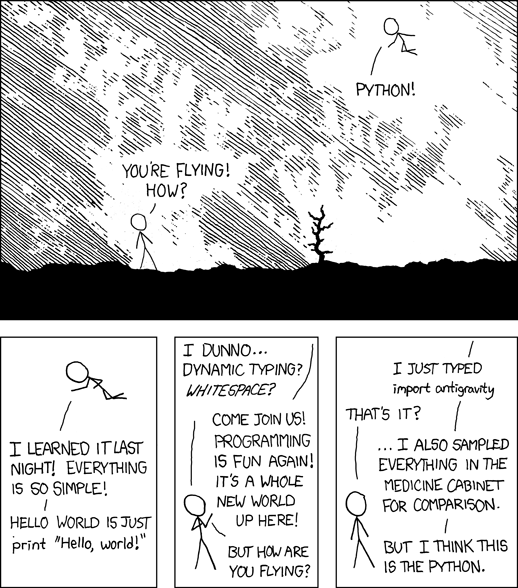
\includegraphics[height=200pt,keepaspectratio]{xkcd_python.png}
    \caption
    {
      Python\footnote{\url{www.xkcd.com/353}} 
    }
    \end{center}
  \end{figure}
\end{frame}
 

\begin{frame}
  \frametitle{PEP 8 Style Guide}
  \begin{enumerate}
    \item 4 spaces per indentation level
  \end{enumerate}
\end{frame}


\begin{frame}
  \frametitle{Hello World}
  \inputminted{python}{hello.py}
\end{frame}


\begin{frame}
  \frametitle{Help}
  Built-in function for getting help on almost \textit{anything} in Python
  \begin{itemize}
    \item Built-in Functions: \lstinline{help(print)}
    \item Variables: \lstinline{foo = "hello"; help(foo)}
    \item Types: \lstinline{help(str)}
    \item Class Functions (Methods): \lstinline{help(str.upper)}
    \item Modules (Files): \lstinline{import string; help(string)}
    \item Reserved Words: \lstinline{help("if")}
    \item Operators: \lstinline{help("**")}
  \end{itemize}
\end{frame}

\begin{frame}
  \frametitle{Closer Look at a Help Page (Function)}
  Let's look at the \texttt{print} function's 
  documentation

  \lstinline{help(print)}

  \begin{itemize}
    \item Signature
    \item Description
    \item Arguments
    \item Optional arguments
    \item Keyword arguments
    \item Default values
  \end{itemize}

\end{frame}


\begin{frame}
  \frametitle{Closer Look at a Help Page (Module)}
  Let's look at the \texttt{string} module's 
  documentation

  \lstinline{import string; help(string)}

  \begin{itemize}
    \item Name (and brief description)
    \item Description (of module variables)
    \item Classes and their methods
    \item Functions
    \item Data (the values of module variables)
    \item File (where the \texttt{string} module is on our system)
   \end{itemize}

\end{frame}

\begin{frame}[fragile]
  \frametitle{Python Idioms: Swap Values}
  \begin{columns}
  \begin{column}{0.5\textwidth}
    \textbf{Python}
    \inputminted{python}{swap.py}
  \end{column}
  \begin{column}{0.5\textwidth}
  \textbf{Naive Java Implementation}
  \begin{lstlisting}
    int a = 1, b = 2;
    int temp = a;
    b = a;
    a = temp;
  \end{lstlisting}
  \end{column}
  \end{columns}
\end{frame}

\begin{frame}[fragile]
  \frametitle{Python Idioms: Exponentiation}
  \textbf{Python}
  \inputminted{python}{exponentiation.py}
  
  \textbf{Naive Java Implementation}
  \begin{lstlisting}
    List<Integer> exp = new ArrayList<>();
    for (int n = 1; n <= 10; n++) {
      Integer nToTheN = Math.pow(n, n);
      exp.add(nToTheN);
    }
  \end{lstlisting}
\end{frame}

\begin{frame}[fragile]
  \frametitle{Python Idioms: Chained Conditions}
  \textbf{Python}
  \inputminted{python}{ordered_units.py}
  
  \textbf{Naive Java Implementation}
  \begin{lstlisting}
    bool areOrderedUnits(double x, double y) {
      return 0 <= x && x < y && y <= 1;
    }
  \end{lstlisting}
\end{frame}
 
\begin{frame}
  \frametitle{Caesar Cipher}
  \inputminted{python}{caesar.py}
\end{frame}


\end{document}

